\documentclass[10pt]{article}
\usepackage[a4paper,margin=2.2cm]{geometry}
\usepackage{amsmath,amssymb}
\usepackage{graphicx}
\usepackage{booktabs}
\usepackage{array}
\usepackage{multirow}
\usepackage{xcolor}
\usepackage{listings}
\usepackage{tikz}
\usetikzlibrary{positioning,arrows.meta,fit,backgrounds}
\usepackage{algorithm}
\usepackage{algpseudocode}
\usepackage{caption}
\usepackage[hidelinks]{hyperref}

\definecolor{codebg}{HTML}{F6F6F4}
\definecolor{kw}{HTML}{2A5DB0}
\definecolor{cm}{HTML}{6B6A66}
\definecolor{st}{HTML}{A3461E}
\lstdefinestyle{qcl}{
  language=Python, basicstyle=\ttfamily\footnotesize, keywordstyle=\color{kw}\bfseries,
  commentstyle=\color{cm}\itshape, stringstyle=\color{st}, backgroundcolor=\color{codebg},
  frame=none, xleftmargin=4pt, framexleftmargin=4pt, columns=fullflexible,
  showstringspaces=false, breaklines=true, aboveskip=6pt, belowskip=6pt,
  morekeywords={with}}
\lstset{style=qcl}

\newcommand{\qpuCost}{285.0}
\newcommand{\qpuCurrency}{CNY}
\newcommand{\qpuJobs}{24}

\IfFileExists{tables/bench_macros.tex}{\newcommand{\benchSequentialautoA}{1.00}
\newcommand{\benchLanesoffA}{1.16}
\newcommand{\benchCompiledoffA}{0.91}
\newcommand{\benchCompiledonA}{1.30}
\newcommand{\benchSequentialautoB}{1.00}
\newcommand{\benchLanesoffB}{1.10}
\newcommand{\benchCompiledoffB}{1.09}
\newcommand{\benchCompiledonB}{1.09}
\newcommand{\benchMqSequential}{1.00}
\newcommand{\benchMqCompiled}{2.12}
}{}

\newcommand{\qcl}{QCL}
\newcommand{\code}[1]{\texttt{#1}}

\title{\Large\textbf{QCL: a placement-explicit dataflow language and compiler\\
for hybrid CPU--GPU--QPU quantum chemistry,\\
with experiments on a 24-qubit superconducting processor}}
\author{ChemFlow project\\\small Draft technical report, \today}
\date{}

\begin{document}
\maketitle

\begin{abstract}
Quantum-chemistry workflows that use a quantum processor are hybrid programs: a mean
field and integrals on GPUs, amplitudes and diagonalizations on CPUs, circuit sampling
on a metered cloud QPU, and an exact reference wherever one is affordable. We describe
\qcl{}, a Python-embedded dataflow language in which every computation states the device
it runs on, every result carries units, uncertainty and provenance, and infeasible or
over-budget programs fail at compile time, before any QPU money is spent. Programs are
traced into a typed intermediate representation held in Rust, checked against a single
table of 103 primitives, planned (transfers, cost, budgets), and then compiled by a
scheduler that removes dead and duplicate nodes, ranks nodes by their critical path and
runs every device lane concurrently, with several CPU worker processes and several
in-flight cloud QPU jobs at once; lanes that do real work run in their own processes.
On the real QPU the compiled schedule halves the wall time of a 20-qubit, four-geometry
experiment. We used the language to run a complete experiment on
the lqcloud MQ02 superconducting processor (24 qubits): CCSD-seeded LUCJ circuits for
H$_2$ and for N$_2$ in active spaces from 4 to 24 qubits, sampled on hardware and on an
ideal simulator, diagonalized by sample-based quantum diagonalization (SQD), and compared
with exact CASCI and with a uniform-random-bitstring control. Hardware samples lose
fidelity to the ideal distribution rapidly with circuit size (Hellinger fidelity
0.73--0.86 at 4 qubits and 11 CZ gates, $\approx 10^{-3}$ at 16 qubits). SQD on hardware
samples nevertheless reaches the exact energy in every active space up to 24 qubits, and
so do uniformly random bitstrings: configuration recovery, spin closure and the
single-excitation extension rebuild the full active-space sector from noise. The language
makes this visible, because SQD results carry their subspace and sector dimensions and
the program can switch the recovery steps off. We report the problems found on the way
and how they were solved, including a non-reproducible orbital choice that changed every
sampled circuit between runs and a job-reuse key that resubmitted (and paid for)
identical circuits.
\end{abstract}

\tableofcontents

%======================================================================================
\section{Problem definition}
\label{sec:problem}

A hybrid quantum-chemistry calculation is a dataflow graph whose nodes run on different
kinds of device. For the sample-based quantum diagonalization (SQD)
workflow~\cite{sqd} of one molecular geometry,
\begin{enumerate}
\item a GPU computes the restricted Hartree--Fock (RHF) mean field;
\item a CPU builds the active-space Hamiltonian and the CCSD amplitudes that seed a
local unitary cluster Jastrow (LUCJ) circuit~\cite{lucj};
\item a QPU samples the circuit;
\item a CPU diagonalizes the Hamiltonian in the subspace spanned by the sampled
configurations;
\item a GPU computes the exact active-space energy (CASCI) as a reference.
\end{enumerate}
A dissociation curve repeats this for many geometries, and an experiment adds controls.
Writing such workflows directly in Python against PySCF, GPU4PySCF, Qiskit and a cloud
SDK leaves four problems to every author:

\begin{description}
\item[P1 Deployment.] Where each step runs and when data moves between devices is
implicit, and a wrong device or a missing implementation is found at run time,
possibly after a paid QPU job.
\item[P2 Honest results.] A number without its unit, uncertainty, method and validity
domain invites wrong comparisons, for example subtracting energies of two different
methods, or reading SQD's batch spread as its error.
\item[P3 Resource control.] Cloud QPUs are metered. Shots, device time and money need
limits that a program cannot raise, forecasts before submission, and a ledger that never
pays twice for the same job.
\item[P4 Performance.] The steps on different devices are independent across
geometries, yet a script runs them one after another. Overlapping GPU, CPU and QPU work
(including the minutes a cloud job waits in a queue) and running independent CPU steps
side by side is where the wall time of a hybrid workflow is won or lost.
\end{description}

\qcl{} addresses P1--P3 in the language and its checker, and P4 in its compiler and
runtime. Section~\ref{sec:language} describes the language, Section~\ref{sec:compiler}
the compilation layer, Section~\ref{sec:impl} the implementation, and
Section~\ref{sec:experiments} the experiments on the MQ02 processor and the F5090
GPU server. Section~\ref{sec:problems} lists the problems found while doing this work
and their solutions.

%======================================================================================
\section{Language design}
\label{sec:language}

\subsection{Programming model}

A \qcl{} program is an ordinary Python function decorated with \code{@qcl.workflow}.
Compiling it does not execute it: the body is \emph{traced}, and each \qcl{} call
records a node in a typed graph held in Rust. There are three kinds of calls:
\emph{compute operations} (\code{qcl.scf.rhf}, \code{qcl.fci.solve}, \code{qcl.sample},
\code{qcl.sqd.diagonalize}, \dots), which must be placed on a device;
\emph{patterns} (\code{qcl.map}, \code{qcl.scan}, \code{qcl.optimize}, \dots), which
distribute callbacks over lanes of devices; and \emph{host operations} (molecule edits,
attribute projections such as \code{.energy} or \code{.hamiltonian}, arithmetic on
estimates, kernel construction), which never need a device. Python control flow runs at
trace time on static metadata; branching on computed values uses patterns
(\code{qcl.cond}, \code{qcl.iterate}).

\paragraph{Placement is the only deployment mechanism.} \code{v.to(x)} declares that
value \code{v} lives on device \code{x}. If the operation producing \code{v} is not yet
placed, it runs on \code{x}; if it is, \code{.to(x)} makes a copy on \code{x}. Every
compute operation must be placed exactly once (QCL-E201), an operation placed on a device
kind without an implementation is an error rather than a silent fallback (QCL-E203), and
with \code{strict\_transfers=True} every device-to-device movement must be an explicit
copy (QCL-E205). Devices are ordinary arguments, so the same program runs on a laptop
or on a four-GPU server by changing the call. Placement, together with device options
such as GPU precision or a lane's slot count, is all the program says about deployment;
the compiler (Section~\ref{sec:compiler}) decides \emph{when} each placed node runs,
never \emph{where}.

\paragraph{Example.} Listing~\ref{lst:hardware} is the program behind the hardware
experiments of Section~\ref{sec:experiments}. For each molecule it computes a GPU mean
field, a CPU active space and CCSD amplitudes, samples the same LUCJ kernel on a
hardware QPU and on an ideal simulator, runs four SQD diagonalizations (each sample set
with and without configuration recovery), and computes the exact CASCI energy on the GPU.
Every cross-device movement is an explicit \code{.to()}.

\begin{lstlisting}[caption={The hardware SQD experiment in \qcl{} (\code{qcl/apps/qpu\_sqd\_experiment.py}).},label=lst:hardware,float=t]
def sqd(space, bits, cpu, **options):
    return qcl.sqd.diagonalize(space.hamiltonian, bits, space.sector, **options).to(cpu)

@qcl.workflow
def hardware_sqd(molecules, cpu, gpus, qpu, simulator, active, shots, ideal_shots, seed=11):
    rows = []
    for index, molecule in enumerate(molecules):
        gpu = gpus[index % len(gpus)]
        mean_field = qcl.scf.rhf(molecule).to(gpu)
        space = qcl.active_space(mean_field.to(cpu), active).to(cpu)
        amplitudes = qcl.ccsd.amplitudes(space).to(cpu)
        kernel = qcl.kernels.lucj(space, params=amplitudes)
        hardware = qcl.sample(kernel, shots=shots, seed=seed + index).to(qpu).to(cpu)
        ideal = qcl.sample(kernel, shots=ideal_shots, seed=seed + index).to(simulator).to(cpu)

        rows.append({
            "rhf": mean_field.energy,
            "casci": qcl.fci.solve(space.hamiltonian.to(gpu), space.sector.to(gpu)).to(gpu).energy,
            "sqd_qpu": sqd(space, hardware, cpu),
            "sqd_qpu_raw": sqd(space, hardware, cpu, recovery=False, extend=False),
            "sqd_sim": sqd(space, ideal, cpu),
            "sqd_sim_raw": sqd(space, ideal, cpu, recovery=False, extend=False),
            "bits_qpu": hardware, "bits_sim": ideal})
    return rows

cloud = qcl.Device("mq02", "qpu", qubits=24, site="remote", billing="metered",
                   provider="lqcloud", backend="MQ02")
plan = hardware_sqd.compile(molecules, cpu, gpus, cloud, simulator, qcl.Active(10, 8),
                            4000, 100000, strict_transfers=True)
print(plan.explain()); print(plan.estimate()); print(plan.schedule()["predicted"])
rows = plan.run(overlap=True)
\end{lstlisting}

\subsection{Types and result semantics}

Values are typed (\code{Molecule}, \code{ScfResult}, \code{ActiveSpace},
\code{FermionOperator}, \code{QubitOperator}, \code{Kernel}, \code{Bitstrings},
\code{Estimate}, \dots). Fermionic and qubit operators are distinct types, so passing a
Jordan--Wigner operator where SQD expects the fermionic Hamiltonian is a compile error
(QCL-E101). Every numerical result is an \code{Estimate}: a value, a statistical
variance, a unit (QCL-E102 on a unit mismatch) and provenance recording the question
(molecule, property, sector), the method (family, basis, active space), the
implementation and library versions, the device and the seeds. Subtracting two energies
from different methods is refused (QCL-E103); this is why the N$_2$ application computes
SQD$-$CASCI after the run, from the two provenance-carrying estimates, rather than inside
the program. SQD estimates also carry the subspace dimension, the sector dimension, the
fraction of samples in the target particle sector, whether recovery and extension were
used, and a validity flag stating that the batch variance does not bound the subspace
bias. These fields are what exposed the main experimental finding of
Section~\ref{sec:experiments}.

\subsection{Resource policy}

QPU limits are set by the operator in a policy file the program cannot override:
\begin{lstlisting}[language={}]
[budget]
qpu_shots = 2000000
wall_time = "6h"
[cloud_qpu]            # metered cloud QPUs only
qpu_cost = 400
currency = "CNY"
\end{lstlisting}
\code{plan.estimate()} forecasts shots, device time and money from a fitted tariff and
timing table before anything runs. A program can only lower limits
(\code{budget=qcl.Budget(...)}); an over-budget plan fails with QCL-E301, and an operator
can require a plan-hash-bound approval above a threshold (QCL-E302). At run time the
MQ02 adapter writes a durable reservation before it submits, attaches to recorded jobs
instead of resubmitting after a lost result, and reuses completed jobs. The reuse key is
discussed in Section~\ref{sec:problems}.

%======================================================================================
\section{The compilation layer}
\label{sec:compiler}

Figure~\ref{fig:pipeline} shows the path from a traced program to execution.

\begin{figure}[t]
\centering
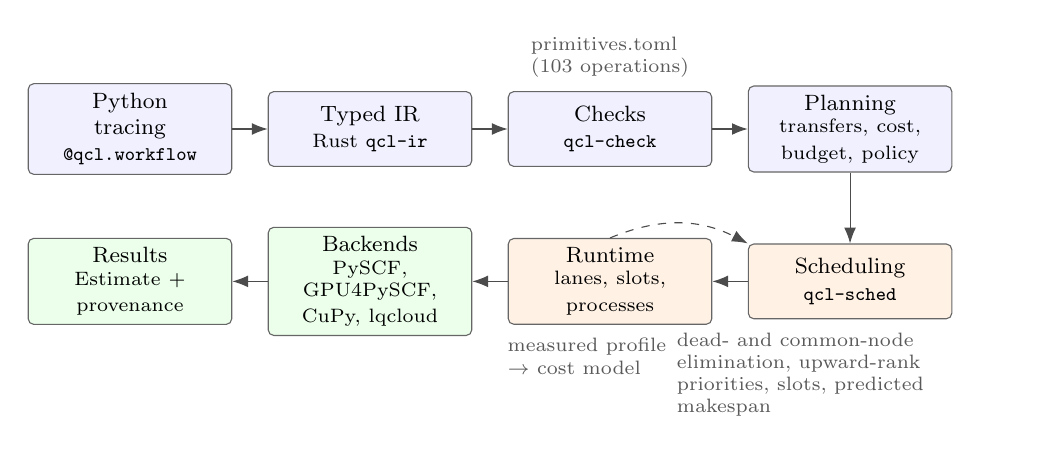
\begin{tikzpicture}[
  box/.style={draw=black!60, rounded corners=2pt, fill=#1, align=center,
              font=\footnotesize, minimum height=0.95cm, text width=2.35cm},
  box/.default={black!3},
  arr/.style={-{Latex[length=2mm]}, black!70},
  note/.style={font=\scriptsize, text=black!65, align=left}]
\node[box={blue!6}] (trace) {Python\\tracing\\\scriptsize\code{@qcl.workflow}};
\node[box={blue!6}, right=0.45cm of trace] (ir) {Typed IR\\\scriptsize Rust \code{qcl-ir}};
\node[box={blue!6}, right=0.45cm of ir] (check) {Checks\\\scriptsize \code{qcl-check}};
\node[box={blue!6}, right=0.45cm of check] (plan) {Planning\\\scriptsize transfers, cost,\\budget, policy};
\node[box={orange!10}, below=0.9cm of plan] (sched) {Scheduling\\\scriptsize \code{qcl-sched}};
\node[box={orange!10}, left=0.45cm of sched] (rt) {Runtime\\\scriptsize lanes, slots,\\processes};
\node[box={green!8}, left=0.45cm of rt] (be) {Backends\\\scriptsize PySCF, GPU4PySCF,\\CuPy, lqcloud};
\node[box={green!8}, left=0.45cm of be] (res) {Results\\\scriptsize Estimate +\\provenance};
\draw[arr] (trace) -- (ir); \draw[arr] (ir) -- (check); \draw[arr] (check) -- (plan);
\draw[arr] (plan) -- (sched); \draw[arr] (sched) -- (rt); \draw[arr] (rt) -- (be);
\draw[arr] (be) -- (res);
\node[note, above=0.05cm of check] {primitives.toml\\(103 operations)};
\node[note, below=0.05cm of sched, text width=4.4cm] {\raggedright dead- and common-node\\elimination, upward-rank\\priorities, slots, predicted\\makespan};
\node[note, below=0.05cm of rt, text width=2.6cm] {\raggedright measured profile\\$\to$ cost model};
\draw[arr, dashed] (rt.north) to[bend left=25] node[note, left, pos=0.45] {} (sched.north west);
\end{tikzpicture}
\caption{The \qcl{} compilation pipeline. Diagnostics from tracing, checking and
planning are collected and reported together, with stable codes, source spans and fix
hints, before anything runs. Measured node durations from each run flow back into the
scheduler's cost model (dashed).}
\label{fig:pipeline}
\end{figure}

\subsection{Tracing and the intermediate representation}

The frontend records each call through a PyO3 graph builder into a Rust graph of nodes
(\code{id}, operation, node kind, value type, inputs, parameters, device, guards, source
span). Node identifiers are a topological order. The graph is versioned and serializable;
its hash ignores source locations, so the same program traced from two files compiles to
the same plan hash, which approval and caching are bound to.

\subsection{One table of primitives}

Every operation the IR can contain is declared once, in \code{primitives.toml}: its node
kind (27 host, 54 compute, 21 projection and one copy operation), its output type, the
device kinds that have an implementation, its parallel axis and optional diagnostic
wording. The Rust checker reads the table for QCL-E203; the graph builder takes node
kinds and output types from it; \code{qcl.compile} refuses a graph that disagrees with
it; and the worker's handlers are registered per operation with
\code{@implements("op")}. A test fails if the table, the registry and the checker
disagree, so adding an operation is three edits: a table entry, a frontend function and a
handler. Conditions that depend on inputs (GPU SCF requires a closed shell, GPU densities
need the CI state on the same GPU, a QPU kernel must fit the device) stay explicit rules
in the checker.

\subsection{Checks and planning}

The checker validates types, units, sectors and model compatibility, the placement rules
and feasibility (memory, qubit counts, simulator hosts). The planner inserts and lists
transfers (\code{plan.explain()}), estimates cost per device (\code{plan.estimate()}),
and checks the operator policy. All errors of one compilation are reported together.

\subsection{Dataflow optimization and scheduling}
\label{sec:sched}

The scheduler, a Rust crate (\code{qcl-sched}), compiles the checked graph into the
schedule that \code{plan.run(overlap=True)} executes. It never changes placement.

\paragraph{Dead-node elimination.} Only nodes that an output or a \code{qcl.require}
check depends on (through inputs or guards) are executed. A QPU job whose result no
output reads is never submitted.

\paragraph{Common-subexpression elimination.} Nodes are compared after their inputs'
duplicates are resolved, by operation, kind, parameters, device, inputs and guards;
a duplicate becomes an alias of the first equal node, so equal chains collapse and a
value copied twice to the same GPU moves once. QPU sampling and estimation are never
merged: each requested job runs.

\paragraph{Priorities.} With predicted costs $c_v$, each node gets its upward rank
\[
  r_v = c_v + \max_{w \in \mathrm{succ}(v)} r_w ,
\]
the predicted time from the start of $v$ to the end of the program along its most
expensive path (as in HEFT list scheduling~\cite{heft}). The maximum rank is the
critical-path length $T_\infty$, a lower bound on any schedule's makespan.

\paragraph{Lanes and slots.} Every device is a \emph{lane}. A lane runs up to $s$ nodes
at once: GPUs and local simulators default to one, a cloud QPU keeps up to four jobs in
flight, and a CPU lane gets as many slots as it has independent nodes at one dependency
depth, bounded by its threads divided by eight. Each CPU node then runs with
$\min(32, T/s)$ OpenMP threads (Section~\ref{sec:problems} explains the cap of 32).
\code{device.with\_options(slots=n)} overrides the default.

\paragraph{Dispatch.} Algorithm~\ref{alg:dispatch} is both the runtime's dispatch loop
and, run on predicted costs, the scheduler's simulation that yields the predicted
makespan reported by \code{plan.schedule()}.

\begin{algorithm}[t]
\caption{Lane dispatch (runtime and predicted-makespan simulation)}
\label{alg:dispatch}
\begin{algorithmic}[1]
\Require executed nodes $V$, aliases $A$, ranks $r$, lane $\ell(v)$, slots $s(\ell)$
\State $\mathrm{need}(v) \gets \{A(u) : u \in \mathrm{inputs}(v) \cup \mathrm{guards}(v)\}$ for all $v \in V$
\State put every $v$ with $\mathrm{need}(v)=\emptyset$ into the ready heap of $\ell(v)$, keyed by $-r_v$
\Loop
  \For{each lane $\ell$}
    \While{$\mathrm{busy}(\ell) < s(\ell)$ and $\mathrm{ready}(\ell) \neq \emptyset$}
      \State start the highest-rank ready node of $\ell$ \Comment{CPU compute $\to$ lane process}
    \EndWhile
  \EndFor
  \If{nothing is running} \textbf{break} \EndIf
  \State wait for the next node $v$ to finish; give its value to its aliases
  \For{$w$ with $v \in \mathrm{need}(w)$}
    \State remove $v$ from $\mathrm{need}(w)$; if empty, push $w$ into $\mathrm{ready}(\ell(w))$
  \EndFor
\EndLoop
\end{algorithmic}
\end{algorithm}

\paragraph{Cost model.} A node's cost signature is its operation, device kind, whether
the device is remote, and the problem sizes it works on (the nearest active space and
molecule above it, its shot count, and SQD's recovery and extension flags). Unmeasured
signatures use size-based estimates (for example, the determinant count times the
square of the orbital count for FCI and SQD). After every run, measured durations are
folded into a per-user profile cache as an exponential moving average, so the second run
of a workflow is scheduled with measured costs. Only nodes that ran alone in their lane
process (or waited on a cloud QPU) are learned from: durations measured in threads that
shared an interpreter include the other lanes' contention. Costs only order work;
results never depend on them.

\paragraph{Runtime: lanes, slots and processes.} A first runtime ran every lane as a
thread pool inside one worker process. The benchmarks showed why that is not enough:
the scientific libraries do much of their work in Python (state preparation for the
simulator, Davidson loops that launch many small GPU kernels, SQD's configuration
handling), so lanes contended for one interpreter lock. With one node per device in
threads, a GPU FCI that takes 1.2\,s alone took 54\,s, and the run was no faster than
sequential execution. The runtime therefore gives every lane that does real work its own
processes (module \code{qcl.\_runtime}):
\begin{itemize}
\item a GPU lane is one persistent process that keeps its values on the GPU;
\item a CPU lane, and a QPU simulator lane, is a pool of stateless processes, one per
slot;
\item cloud-QPU lanes, which mostly wait on the network, and host operations stay in
threads of a coordinator.
\end{itemize}
Processes are spawned once per run and started while the first nodes execute. A value
moves only when a node in another process needs it, serialized with cloudpickle; arrays
go through a content-addressed artifact store in shared memory (\code{/dev/shm}) with
atomic writes. A value that cannot leave its GPU process (CuPy arrays, CUDA handles)
stays resident there, and nodes that read it --- a projection, or an explicit copy to the
host --- are routed to that process. GPU data therefore leave the device only through an
explicit copy, as the language promises. Conversely, a host copy must hold no device
data: the copy handler drops private GPU caches that GPU4PySCF leaves on converted
objects, and a host value that still cannot leave a GPU process is reported in the
profile (QCL-W202), because it would silently pull its consumers into that process.
\code{QCL\_TRACE} records every dispatch and completion, and SIGUSR1 dumps the stacks
of every lane process. Handlers rely on object identity (an operator
and a sector must belong to the \emph{same} active space), so the transport preserves it:
every non-trivial object gets a token, a process that already holds an object receives a
reference instead of a copy, results that contain objects the coordinator sent resolve
back to the originals, and tokens are recorded as held only once a message has been
serialized successfully. The sentinel for guarded-off values pickles by reference, so it
stays a singleton in every process. The scheduler enables lane processes for a lane
predicted to be busy for at least two seconds.

\paragraph{Schedule invariance.} Results must not depend on the schedule. The tests
compare sequential, threaded and process execution to $10^{-10}$\,Eh, and the
experiments in Section~\ref{sec:bench} check it on every benchmark run.
Section~\ref{sec:problems} describes the non-determinism this exposed upstream of the
scheduler and how it was removed.

%======================================================================================
\section{Implementation}
\label{sec:impl}

The core is about 4,300 lines of Rust in five crates: \code{qcl-ir} (graph, types,
primitive table), \code{qcl-check} (checks and diagnostics), \code{qcl-cluster} (cluster
and device files), \code{qcl-ci} (a native determinant CI engine) and \code{qcl-sched}
(the scheduler above), plus the PyO3 module. The Python frontend and worker are about
7,900 lines, including 13 handler modules. Scientific work is delegated to existing
libraries through ChemFlow's adapters: PySCF~2.14 (SCF, CASCI, CCSD, selected CI),
GPU4PySCF~1.8 (GPU SCF), CuPy (GPU FCI and statevector sampling), Qiskit (transpilation to
MQ02's \code{rz, sx, x, cz} basis) and the lqcloud SDK for MQ02.

\paragraph{Platform.} All runs used the F5090 server: four NVIDIA RTX~5090 GPUs
(sm\_120, driver 595 / CUDA~13), 768 CPU cores and Ubuntu~24.04. The QPU is lqcloud's
MQ02 ("AGate~100" chip, 24 qubits on a linear coupling chain; calibration of
2026-11-20: median CZ fidelity 0.9956 (0.9920--0.9983), median readout fidelities 0.992
for $|0\rangle$ and 0.981 for $|1\rangle$, median $T_1$ 63\,\textmu s, $T_2$ 9.9\,\textmu s,
$T_2^{*}$ 3.9\,\textmu s). Circuits are mapped to the best-scoring contiguous chain of the
device, without readout correction or other error mitigation.

%======================================================================================
\section{Experiments}
\label{sec:experiments}

\subsection{Protocol}

For H$_2$/STO-3G (2 electrons in 2 orbitals, 4 qubits, six bond lengths) and for
N$_2$/cc-pVDZ in five active spaces --- (4,4), (6,6), (10,8), (10,10) and (12,12), that is
8, 12, 16, 20 and 24 qubits --- the program of Listing~\ref{lst:hardware} ran with
1000 (H$_2$), 4000 (N$_2$ up to 16 qubits), 8000 (20 qubits) or 2000 (24 qubits) hardware
shots per geometry and 100,000 ideal shots. For every geometry we report:
\begin{itemize}
\item the Hellinger fidelity $F_\mathrm{H} = (\sum_x \sqrt{p_x q_x})^2$ between the
hardware and ideal bitstring distributions;
\item the fraction of hardware shots in the target $(N_\alpha, N_\beta)$ sector;
\item SQD energies from hardware and ideal samples, with configuration recovery and the
single-excitation extension (``full'', the default) and without them (``samples only'');
\item a control outside the \qcl{} program: SQD on as many uniformly random bitstrings as
hardware shots;
\item the exact CASCI energy and the RHF energy.
\end{itemize}
The planned experiments used 24 MQ02 jobs and cost \qpuCost{} \qpuCurrency{}. A
first scheduling benchmark then resubmitted circuits it was meant to reuse (22 further
jobs, 405\,CNY), which exposed the job-reuse problem of Section~\ref{sec:problems}; the
final hardware benchmark used 8 jobs (60\,CNY).

\subsection{Hardware fidelity}

\begin{figure}[t]
\centering
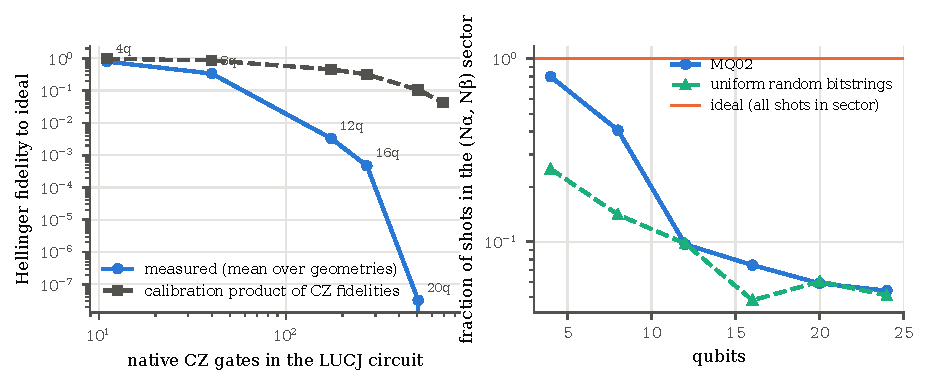
\includegraphics[width=\textwidth]{figures/hardware_fidelity.pdf}
\caption{Left: Hellinger fidelity of MQ02 samples to the ideal distribution against the
number of native CZ gates in the transpiled LUCJ circuit (mean over geometries), with
the product of the calibrated CZ fidelities along the circuit for comparison. The
24-qubit point (690 CZ) is below the plotted range. Right: fraction of shots in the
target particle sector, against the same fraction for uniformly random bitstrings.}
\label{fig:fidelity}
\end{figure}

Figure~\ref{fig:fidelity} shows the device's output degrading quickly with circuit size.
At 4 qubits (11 CZ gates) the fidelity is 0.73--0.86 and 73--86\% of shots are in the
right particle sector. At 8 qubits (40 CZ) the fidelity is 0.31--0.36. From 12 qubits (174 CZ)
on it is below $10^{-2}$, and the sector fraction is close to that of uniformly random
bitstrings. The product of calibrated CZ fidelities (0.45 at 174 CZ, 0.32 at 270)
overestimates the measured fidelity by orders of magnitude: with $T_2 \approx 10$\,\textmu s
and $T_2^{*} \approx 4$\,\textmu s, decoherence over the circuit depth, not the two-qubit
gate error alone, limits these circuits.

\subsection{Energies}

\begin{figure}[t]
\centering
\begin{minipage}[t]{0.49\textwidth}\centering
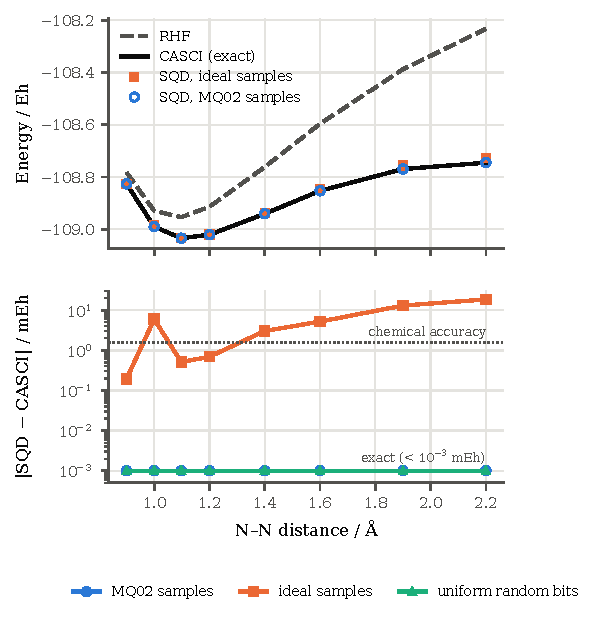
\includegraphics[width=\linewidth]{figures/curve_n2_108.pdf}
\end{minipage}\hfill
\begin{minipage}[t]{0.49\textwidth}\centering
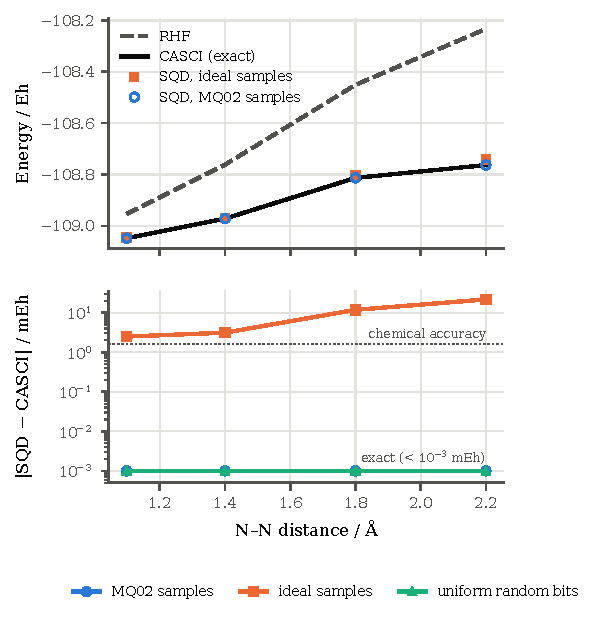
\includegraphics[width=\linewidth]{figures/curve_n2_1010.pdf}
\end{minipage}
\caption{N$_2$/cc-pVDZ dissociation in CAS(10,8) (left, 16 qubits, eight geometries)
and CAS(10,10) (right, 20 qubits, four geometries). Top: RHF, exact CASCI, and SQD from
ideal and MQ02 samples. Bottom: SQD error against CASCI; errors below $10^{-3}$\,mEh are
drawn at the floor.}
\label{fig:curves}
\end{figure}

\begin{table}[t]
\centering
\caption{N$_2$ CAS(10,8), 16 qubits, 4000 MQ02 shots per geometry. SQD with recovery
and extension. $F_\mathrm{H}$: Hellinger fidelity of MQ02 samples; valid: fraction of
MQ02 shots in the sector; dim./sector: SQD subspace dimension over the sector dimension
for MQ02 samples.}
\label{tab:n2108}
\small
\begin{tabular}{rrrrrrrr}
\toprule
$R$/\AA & $E_\mathrm{CASCI}$/Eh & \multicolumn{3}{c}{SQD $-$ CASCI / mEh} & $F_\mathrm{H}$ & valid & dim./sector \\
\cmidrule(lr){3-5}
 & & MQ02 & ideal & uniform & & & \\
\midrule
0.900 & -108.826629 & 0.00 & 0.20 & 0.00 & 0.001 & 0.072 & 3136/3136 \\
1.000 & -108.990330 & 0.00 & 6.01 & 0.00 & 0.000 & 0.075 & 3136/3136 \\
1.098 & -109.034407 & 0.00 & 0.51 & 0.00 & 0.000 & 0.079 & 3136/3136 \\
1.200 & -109.021274 & 0.00 & 0.70 & 0.00 & 0.001 & 0.080 & 3136/3136 \\
1.400 & -108.941001 & 0.00 & 3.04 & 0.00 & 0.001 & 0.080 & 3136/3136 \\
1.600 & -108.852985 & 0.00 & 5.23 & 0.00 & 0.001 & 0.069 & 3136/3136 \\
1.900 & -108.769529 & 0.00 & 13.11 & 0.00 & 0.000 & 0.072 & 3136/3136 \\
2.200 & -108.745355 & 0.00 & 18.67 & 0.00 & 0.000 & 0.069 & 3136/3136 \\
\bottomrule
\end{tabular}

\end{table}

\begin{table}[t]
\centering
\caption{N$_2$ CAS(10,10), 20 qubits, 8000 shots (top), and CAS(12,12), 24 qubits,
2000 shots (bottom). Columns as in Table~\ref{tab:n2108}.}
\label{tab:n2big}
\small
\begin{tabular}{rrrrrrrr}
\toprule
$R$/\AA & $E_\mathrm{CASCI}$/Eh & \multicolumn{3}{c}{SQD $-$ CASCI / mEh} & $F_\mathrm{H}$ & valid & dim./sector \\
\cmidrule(lr){3-5}
 & & MQ02 & ideal & uniform & & & \\
\midrule
1.098 & -109.048064 & 0.00 & 2.48 & 0.00 & 0.000 & 0.064 & 63504/63504 \\
1.400 & -108.972005 & 0.00 & 3.12 & 0.00 & 0.000 & 0.059 & 63504/63504 \\
1.800 & -108.813194 & 0.00 & 11.78 & 0.00 & 0.000 & 0.056 & 63504/63504 \\
2.200 & -108.763293 & 0.00 & 21.59 & 0.00 & 0.000 & 0.059 & 63504/63504 \\
\bottomrule
\end{tabular}
\\[4pt]
\begin{tabular}{rrrrrrrr}
\toprule
$R$/\AA & $E_\mathrm{CASCI}$/Eh & \multicolumn{3}{c}{SQD $-$ CASCI / mEh} & $F_\mathrm{H}$ & valid & dim./sector \\
\cmidrule(lr){3-5}
 & & MQ02 & ideal & uniform & & & \\
\midrule
1.098 & -109.059453 & 0.00 & 1.24 & 0.00 & 0.000 & 0.047 & 853776/853776 \\
2.200 & -108.776827 & 0.00 & 2.53 & 0.00 & 0.000 & 0.061 & 853776/853776 \\
\bottomrule
\end{tabular}

\end{table}

Figure~\ref{fig:curves} and Tables~\ref{tab:n2108}--\ref{tab:n2big} show the result
that matters most for interpreting SQD on this hardware. With the default
post-processing, SQD on MQ02 samples reproduces the exact CASCI energy (error below
$10^{-3}$\,mEh) at every geometry of every active space, including the stretched bonds
where CASCI lies 0.5\,Eh below RHF. SQD on \emph{ideal} samples is worse: 0.2--19\,mEh
in CAS(10,8), 2.5--22\,mEh in CAS(10,10), and 1.2--2.5\,mEh in CAS(12,12). The reason is
in the subspace dimensions: for MQ02 samples the subspace is the entire sector (3136 of
3136 determinants in CAS(10,8), 63\,504 of 63\,504 in CAS(10,10), 853\,776 of 853\,776 in
CAS(12,12)). The ideal LUCJ distribution is concentrated on a few dozen configurations
near the Hartree--Fock determinant, so its subspace is a small part of the sector. Noise
spreads the hardware samples over all configurations, and the post-processing turns them
into the whole sector.

\subsection{Ablation: what the samples contribute}

\begin{figure}[t]
\centering
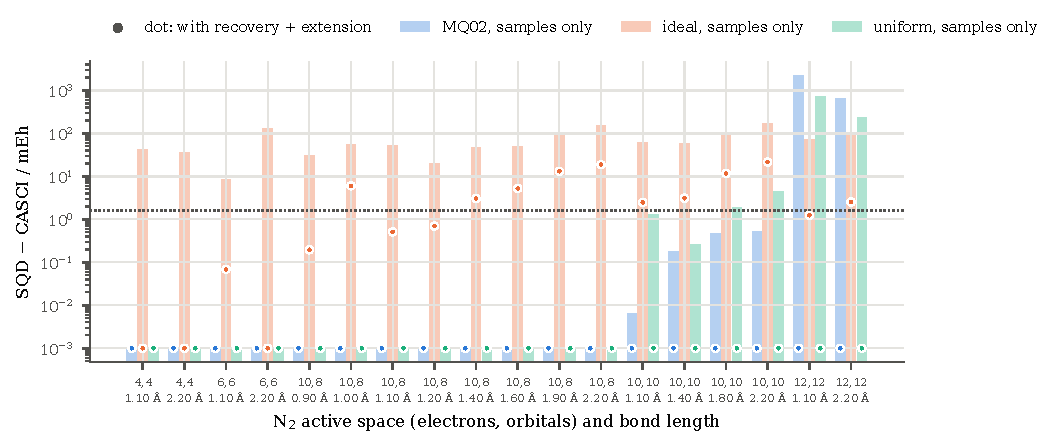
\includegraphics[width=\textwidth]{figures/ablation.pdf}
\caption{SQD error for every N$_2$ geometry. Bars: subspace from the sampled valid
configurations only (no recovery, no extension); dots: with recovery and extension.
Blue: MQ02 samples; orange: ideal samples; green: uniformly random bitstrings. Values
below $10^{-3}$\,mEh are drawn at the floor.}
\label{fig:ablation}
\end{figure}

Figure~\ref{fig:ablation} separates the device's contribution from the
post-processing's. With recovery and extension (dots), MQ02 samples and uniformly random
bitstrings both reach the exact energy everywhere. Only ideal samples do not, because
they are too concentrated. Without recovery and extension (bars), the result depends on
whether the valid samples alone can span the sector. Up to 16 qubits they do: the
$\alpha$ and $\beta$ strings of a few hundred valid shots already cover every string,
and spin closure of the string sets gives the full product space. At 20 qubits the raw
subspaces are partial and errors are 0.006--0.5\,mEh for MQ02 and 0.3--4.4\,mEh for
uniform bitstrings. At 24 qubits the raw subspaces cover 3--5\% of the sector, and the
energies are 0.7--2.3\,Eh above CASCI: far above RHF, and, at 1.1\,\AA, worse for MQ02
samples (2261\,mEh) than for uniform bitstrings (708\,mEh). The valid configurations
the device produces are biased toward high-energy determinants, not toward the
low-energy ones the circuit prepares.

\paragraph{Interpretation.} For these active spaces and this device, the SQD energy is a
property of the classical post-processing, not of the quantum computer: configuration
recovery fills the particle sector from any bitstrings, spin closure squares the number
of strings, and the extension adds every single excitation of the leading
configurations. Reported alone, a near-exact SQD energy would suggest a working quantum
pipeline. The subspace and sector dimensions in the provenance, the
\code{recovery=False, extend=False} switch, and a uniform-bitstring control show that it
is not. Meaningful hardware SQD needs active spaces whose sectors are far larger than
what recovery and closure can fill from the shot budget, and circuits shallow enough
that the device's distribution keeps measurable overlap with the ideal one.

\paragraph{H$_2$.} With 4 qubits every subspace is the full 4-determinant sector, so all
SQD energies are exact. The 4-qubit circuit is the only one in which the hardware
distribution is close to the ideal one (Figure~\ref{fig:h2}).

\begin{figure}[t]
\centering
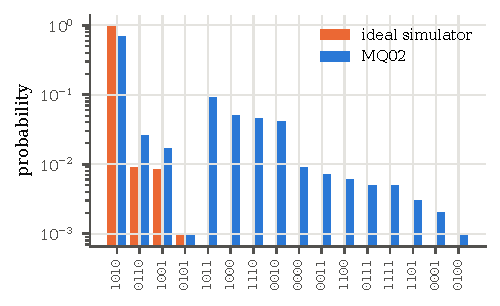
\includegraphics[width=0.48\textwidth]{figures/distribution_h2_22.pdf}
\caption{H$_2$/STO-3G at 0.74\,\AA: measured MQ02 and ideal bitstring probabilities
(qubit 0 first; $\alpha$ then $\beta$ spin orbitals). Hellinger fidelity 0.725.}
\label{fig:h2}
\end{figure}

\subsection{Scheduling performance}
\label{sec:bench}

The same programs were run four ways on F5090: sequentially (one node at a time),
with lanes (every device concurrently, one node per device, all in threads), with the
compiled schedule in threads (lanes, slots and priorities), and with the compiled
schedule and CPU lane processes. To isolate the classical scheduling from the QPU queue,
these runs used a second GPU statevector simulator in place of MQ02. A final pair of runs
used MQ02 with new jobs in each mode, to include real QPU latency.
Table~\ref{tab:bench} reports wall time, the sum of node durations, the scheduler's
predicted makespan and the speed-up over sequential execution.

\begin{table}[t]
\centering
\caption{Execution of the hardware-SQD program under four schedules. ``Node time'' is
the sum of the measured node durations; ``predicted'' is the scheduler's makespan
from its cost model; $|\Delta E|$ is the largest difference in RHF and CASCI energies
against the sequential run.}
\label{tab:bench}
\small
\resizebox{\textwidth}{!}{\IfFileExists{tables/bench.tex}{\begin{tabular}{lrrrrrr}
\toprule
Workload & execution & wall/s & node time/s & predicted/s & speed-up & max $|\Delta E|$/Eh \\
\midrule
N$_2$ CAS(10,10), 4 geometries & sequential & 14.0 & 12.1 &  & 1.00$\times$ & 0.0e+00 \\
 & lanes (threads) & 12.0 & 18.7 & 11.2 & 1.16$\times$ & 5.7e-14 \\
 & compiled (threads) & 15.3 & 131.1 & 1.8 & 0.91$\times$ & 8.5e-14 \\
 & compiled (lane processes) & 10.7 & 17.1 & 1.8 & 1.30$\times$ & 1.1e-13 \\
\midrule
N$_2$ CAS(12,12), 2 geometries & sequential & 164.5 & 162.5 &  & 1.00$\times$ & 0.0e+00 \\
 & lanes (threads) & 150.1 & 172.0 & 76.9 & 1.10$\times$ & 9.9e-14 \\
 & compiled (threads) & 150.7 & 192.1 & 76.9 & 1.09$\times$ & 9.9e-14 \\
 & compiled (lane processes) & 151.3 & 164.2 & 76.9 & 1.09$\times$ & 9.9e-14 \\
\midrule
MQ02, CAS(10,10), 4 geometries, new jobs & sequential & 80.4 & 77.6 &  & 1.00$\times$ & -- \\
 & compiled (lane processes) & 38.0 & 104.3 & 15.8 & 2.12$\times$ & -- \\
\bottomrule
\end{tabular}
}{}}
\end{table}

\begin{figure}[t]
\centering
\IfFileExists{figures/bench_timeline.pdf}{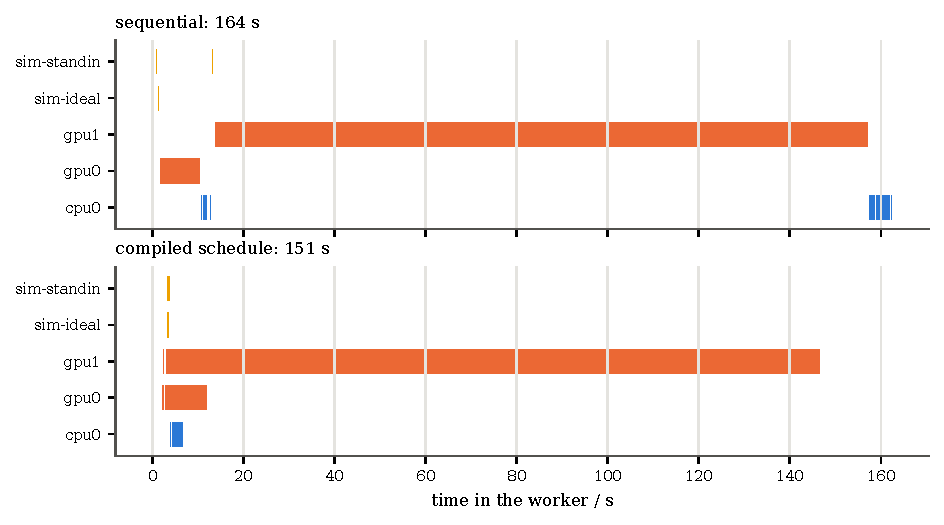
\includegraphics[width=\textwidth]{figures/bench_timeline.pdf}}{}
\caption{Per-lane timelines of the CAS(12,12) program (two geometries): sequential
(top) and compiled with lane processes (bottom). Each bar is one node.}
\label{fig:timeline}
\end{figure}

\paragraph{Results.} On MQ02 the compiled schedule halves the wall time of the
CAS(10,10) program (80.4\,s $\to$ 38.0\,s, $2.12\times$): the four hardware jobs wait
in flight together (11--13\,s each) while the GPU computes mean fields and CASCI and
the CPU lane runs the first SQD diagonalizations in parallel processes. With a simulator
in place of the QPU, the remaining gains are bounded by the critical path. In CAS(12,12)
one GPU FCI of the stretched geometry takes 144\,s and starts 2.8\,s into the run; the
compiled run finishes at 151\,s, so nothing else delays it (Figure~\ref{fig:timeline}).
In CAS(10,10) the whole program takes 14\,s and process start-up costs about 3\,s of it.
All schedules give the same energies to $10^{-13}$\,Eh.

The numbers before the last two fixes of Table~\ref{tab:problems} show where the time
had gone. With the original state preparation (140\,s per 24-qubit sample), threaded
lanes and threaded compiled schedules were no faster than sequential execution
(730, 696 and 704\,s for CAS(12,12)) because every lane contended for one interpreter;
lane processes brought it to 438\,s, and only after the GPU-cache leak was found did the
simulator lanes really run side by side. The largest single gain, however, was
algorithmic: factorizing the LUCJ orbital rotation by spin made state preparation 360
times faster and the sequential CAS(12,12) run 4.4 times faster (730\,s $\to$ 165\,s).
A scheduler can only hide work; the profile it records is what shows which work to
remove. The cost model is the weakest part: it predicted 77\,s for the 144\,s FCI,
because the size-based estimate does not know that Davidson iterations multiply at
stretched geometries.

%======================================================================================
\section{Problems found and their solutions}
\label{sec:problems}

Table~\ref{tab:problems} lists the problems this work ran into, in the order they
appeared. Several were latent in the codebase and surfaced only on new hardware, under
concurrency, or when results were compared run against run.

\begin{table}[p]
\centering
\caption{Problems found while building and running the system, and their solutions.}
\label{tab:problems}
\small
\renewcommand{\arraystretch}{1.15}
\begin{tabular}{>{\raggedright\arraybackslash}p{0.29\textwidth}>{\raggedright\arraybackslash}p{0.32\textwidth}>{\raggedright\arraybackslash}p{0.32\textwidth}}
\toprule
Problem & Cause & Solution \\
\midrule
Every GPU kernel failed on the RTX~5090 (\code{CUDA\_ERROR\_NO\_BINARY\_FOR\_GPU}). &
GPU4PySCF loads cuSOLVER by name and picked up the system CUDA~12.0 toolkit, which
predates sm\_120; CuPy then reused the loaded NVRTC. &
Resolve NVRTC from the CUDA~13 wheels before importing GPU4PySCF; a \code{gpu-cuda13}
extra pins the matching wheels. \\
SCF crashed on GPUs 1--3 (illegal address). &
GPU4PySCF spreads one SCF over all visible GPUs and assumes device 0 leads. &
Import GPU4PySCF in single-device mode; \qcl{} keeps each SCF on the GPU it was placed on. \\
CCSD failed inside long-lived processes. &
Beyond 4\,GB resident memory PySCF switched to an out-of-core path that fails on
integral-only molecules. &
Force in-core integrals (\code{incore\_anyway}); regression test with a mocked memory size. \\
Different bitstrings, LUCJ circuits and SQD energies from run to run. &
SCF fixes orbitals only up to rotations inside degenerate blocks ($\pi$, $\delta$ pairs of
N$_2$) and signs; the eigensolver's choice varied. &
Canonicalize: rotate each degenerate block to diagonalize a fixed symmetry-breaking
operator (s-type probe functions at generic points) and fix signs. Runs are now
reproducible and schedule-invariant. \\
Every rerun resubmitted and paid for identical MQ02 jobs. &
The reuse key hashed the circuit's floating-point angles, which differ by $\sim10^{-10}$
between runs (GPU SCF accumulates with atomics). &
Match recorded jobs by circuit structure, shots and repetition, with angles equal within
$10^{-6}$\,rad. \\
Concurrent lanes were no faster than sequential execution. &
Lanes were threads of one process; Python-level work in the simulator, GPU and SQD code
contended for the interpreter lock (a 1.2\,s GPU FCI took 54\,s). &
Lane processes: one persistent process per GPU (values stay resident), process pools for
CPU and simulator lanes, an identity-preserving transport and a shared-memory store. \\
With lane processes, independent lanes still ran one after another. &
GPU4PySCF's \code{to\_cpu()} leaves private GPU caches (\code{\_opt\_jengine}) on the
host mean field; the host copy could not leave the GPU process, and every consumer was
routed into it. &
Host copies drop private device caches; a node whose host value stays on a GPU is
flagged in the profile (QCL-W202). Found with per-process stack dumps on SIGUSR1. \\
A 24-qubit simulator sample took 140\,s. &
The LUCJ state was built by Python loops over all 853\,776 determinants for each of 132
excitation operators. &
Apply the orbital rotation as $C \to E_\alpha C E_\beta^{\mathsf T}$ on the
$\alpha\times\beta$ string matrix (spin factorization) and vectorize the Jastrow phases:
0.4\,s, equal to the old construction to $10^{-12}$. \\
The scheduler's predictions drifted upward after concurrent runs. &
The cost model learned durations measured in threads that contended for one interpreter. &
Learn only from nodes that ran alone in their lane process (or waited on a cloud QPU). \\
Segmentation fault in PySCF selected CI. &
PySCF's selected-CI kernels crash with several hundred OpenMP threads (768-core host). &
At most 32 OpenMP threads per node; slots share the remaining cores. \\
Protein--ligand MM/GBSA turned from $-15$ to $+12.9$\,kcal/mol in a new environment. &
An unrelaxed 1.6\,\AA{} H--H contact between added hydrogens at the interface. &
Relax hydrogens within 8\,\AA{} of the ligand (others fixed) before the single point;
record the evaluated structure. \\
An ADAPT-VQE test passed alone and failed in the full suite (110\,mEh). &
RHF of square H$_4$ starts from a symmetric guess and stopped either at the stable
solution or at a D$_{4h}$ saddle point 88\,mEh higher, depending on OpenMP reduction
order; ADAPT from the saddle stalls. &
Follow internal (RHF$\to$RHF) instabilities to a stable solution after every RHF;
ADAPT also breaks gradient ties by operator index. \\
HCN/HNC transition-state search no longer converged. &
tblite~0.8 changed GFN2-xTB results the NEB settings were validated on. &
Constrain \code{tblite<0.8}. \\
File reads failed under an ASCII locale. & Locale-dependent default encoding. &
Explicit UTF-8 everywhere. \\
\bottomrule
\end{tabular}
\end{table}

%======================================================================================
\section{Limitations and future work}

\begin{itemize}
\item \textbf{Hardware chemistry.} No error mitigation was used, and the LUCJ circuits
are compiled for a linear chain with a full Givens network per layer. Hardware SQD with
signal requires shallower circuits (fewer layers, truncated rotations,
hardware-native ans\"atze), readout mitigation, and active spaces whose sectors are far
larger than recovery can fill. The uniform control should be part of every such
experiment.
\item \textbf{Runtime.} Values cross processes by serialization and arrays through a
shared-memory file store; a GPU value can reach another GPU only through the host. Zero-copy
exchange between GPU processes (CUDA IPC, DLPack), persistent lane processes across runs
(start-up costs about 3\,s per run), and splitting single nodes along their parallel axes
(determinant blocks, shots) across devices are the next steps; the last would attack the
critical path that now bounds the simulator benchmarks.
\item \textbf{Cost model.} Predictions for unmeasured nodes are coarse, and the
predicted makespan ignores contention between lanes that share a GPU or memory
bandwidth.
\item \textbf{Accounting.} A CPU-time limit applies to the coordinator process;
lane processes are accounted after the run through the operating system's child
resource usage, not interrupted when they exceed it.
\end{itemize}

\section{Conclusion}

\qcl{} makes hybrid CPU--GPU--QPU chemistry programs explicit about where they run,
honest about what their numbers mean, bounded in what they may spend, and fast through a
scheduler that overlaps devices and parallelizes independent work while leaving
placement to the program. Applied to SQD on a 24-qubit superconducting processor, the
same explicitness turned a seemingly excellent result --- exact energies at every
geometry --- into a measured statement: at these circuit sizes the device's samples
carry no usable signal, and the energies come from classical post-processing that
uniformly random bitstrings drive equally well.

\begin{thebibliography}{9}
\bibitem{sqd} J.~Robledo-Moreno \emph{et al.}, ``Chemistry beyond the scale of exact
diagonalization on a quantum-centric supercomputer'', \emph{Sci. Adv.} \textbf{11},
eadu9991 (2025).
\bibitem{lucj} M.~Motta \emph{et al.}, ``Bridging physical intuition and hardware
efficiency for correlated electronic states: the local unitary cluster Jastrow
ansatz for electronic structure'', \emph{Chem. Sci.} \textbf{14}, 11213 (2023).
\bibitem{heft} H.~Topcuoglu, S.~Hariri and M.-Y.~Wu, ``Performance-effective and
low-complexity task scheduling for heterogeneous computing'', \emph{IEEE Trans.
Parallel Distrib. Syst.} \textbf{13}, 260 (2002).
\end{thebibliography}

\appendix
\section{Reproducing the results}

All commands run from the repository root on a machine with the \code{gpu-cuda13} and
\code{qpu} extras installed and \code{LQCLOUD\_API\_KEY} set.
\begin{lstlisting}[language=bash]
export QCL_POLICY_FILE=qcl/apps/qpu-experiment-policy.toml OMP_NUM_THREADS=32
python qcl/apps/qpu_sqd_experiment.py --system h2 --active 2 2 \
    --distances 0.5 0.74 1.0 1.5 2.0 2.5 --shots 1000 --qpu mq02 --overlap --json h2.json
python qcl/apps/qpu_sqd_experiment.py --system n2 --active 10 8 \
    --distances 0.9 1.0 1.098 1.2 1.4 1.6 1.9 2.2 --shots 4000 --qpu mq02 --overlap \
    --json n2_108.json
# ... (4,4), (6,6), (10,10) and (12,12) likewise; then
python docs/paper/analysis.py h2.json n2_44.json n2_66.json n2_108.json \
    n2_1010.json n2_1212.json --calibration mq02_calibration.json --out docs/paper
python docs/paper/bench.py runs/qpu/bench2 --out docs/paper
\end{lstlisting}
The experimental data were recorded before the final orbital canonicalization
(Section~\ref{sec:problems}) replaced a second-moment operator with probe functions,
because the former leaves $\delta$ pairs ambiguous. Rerunning samples circuits in which
degenerate $\pi$ pairs are oriented differently; energies are unaffected and the
conclusions do not depend on the orientation.

\end{document}
